\newpage
\section{Results}
\label{sec:results}
In this section the details of the experimental setup will be presented such that the precision of the depth reconstruction can be computed. Then, illustrations of the algorithm used to find the centroids of the laser dots will be shown in different scenarios. Finally, the point cloud reconstructions of two different objects will be presented.\\

Measurements from the experimental setup displayed in figure \ref{fig:setup1} are:
\begin{equation}
    b = 0.649 \text{ m} \hspace{1cm} z = 1.136 \text{ m}
\end{equation}
Which using equation \ref{eq:phi} yields the camera angle:
\begin{equation}
    \phi = \arctan{\left(\frac{z}{b}\right)} = 60.261^{\text{o}}
\end{equation}
 
In this assignment, video footage of 1920x1080 resolution is used for the reconstruction, which is less than the 6000x4000 maximum resolution supported by the camera sensor. It is assumed that the 1920x1080 resolution is achieved by the camera by simply using a smaller area of the image sensor. The pixel width $p_{w}$ and height $p_{h}$ is thus the full sensor width $s_{w}$ and height $s_{h}$ divided by the maximum resolution.
\begin{equation}
        p_{w} = \frac{22.3 \cdot 10^{-4} \text{ m}}{6000} = 3.71 \cdot 10^{-6} \text{ m}
\end{equation}
\begin{equation}
    p_{h} = \frac{14.9 \cdot 10^{-4} \text{ m}}{4000} = 3.72 \cdot 10^{-6} \text{ m}
\end{equation}

The focal length $f$ is computed using equation \ref{eq:fxfy} where the scaling factors $k_{u}$ and $k_{v}$ are the inverse of the pixel size of the camera along $u$ and $v$, and the focal length in pixels $f_{x}$ and $f_{y}$ are found from the camera calibration matrix. From calibration, it is found that:
\begin{equation}
    f_{x} = 4804 \text{ pixels} \hspace{1cm} f_{y} = 4794 \text{ pixels}
\end{equation}
which yields the focal length $f$:
\begin{equation}
    f = \frac{f_{x}}{k_{u}} = 4804 \cdot 3.71 \cdot 10^{-6} = 17.87 \text{ mm}
\end{equation}
\begin{equation}
    f = \frac{f_{y}}{k_{v}} = 4794 \cdot 3.72 \cdot 10^{-6} = 17.79 \text{ mm}
\end{equation}
As can be seen, the focal lengths computed are very similar. The focal length found using the pixel width is mostly of interest since the depth difference is assumed to only stem from the translation of the laser dots along the horizontal axis in the camera image.\\

Now the theoretical maximum depth resolution $\rho$ can be found as the depth change corresponding to a shift of a single pixel in $u$ as:
\begin{equation}
    \rho = z - b \tan{\left( \phi - \arctan{\left( \frac{1}{k_{u} f} \right)} \right)} = 0.547 \text{ mm}
\end{equation}
Assuming zero image noise which of course is not the case.\\ 

It is now possible to create a 3D reconstruction of the first object of interest, which is the cross-shaped object mentioned throughout this report. The dimensions of this object are illustrated in figure \ref{fig:crossdimensions}, note that the illustration is not to scale. The object in figure \ref{fig:crossdimensions} is symmetric and square such that only three length measurements are required to define the shape. 
 
\begin{figure}[h]
    \centering
    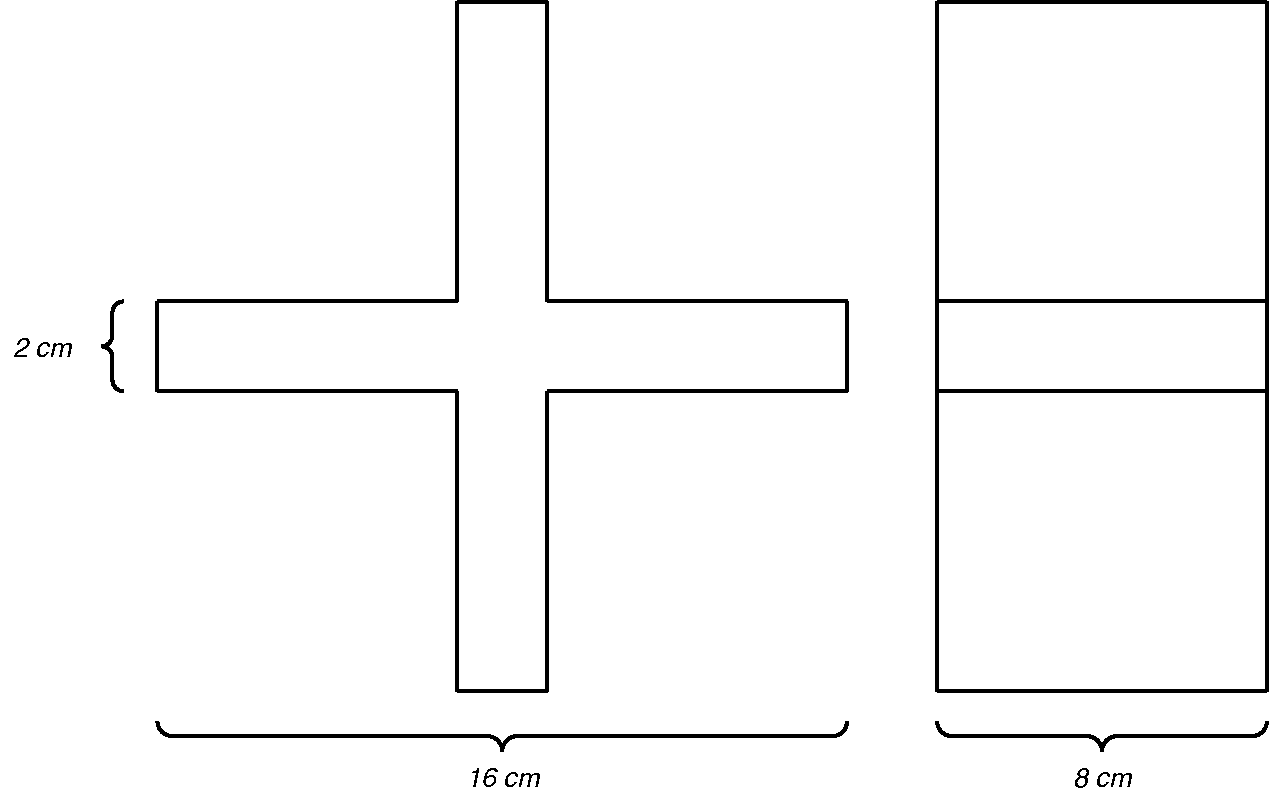
\includegraphics[width=0.73\textwidth]{figures/reconstruction/crossdimensions.pdf}
    \caption{Illustration of the cross-shaped object showing the dimensions. The left subplot shows the object from the front and the right shows the object from above.}
    \label{fig:crossdimensions}
\end{figure}

As also explained in section \ref{sec:reconstructionmath} the cross is placed on top of a cylindrical wooden block on the rotation stage and rotated 360 degrees. A laser then projects a series of laser dots in a vertical pattern onto the object while a camera captures footage of a complete rotation. The resulting video is then analysed frame by frame and the centroids of the laser dots in pixel coordinates are found in Matlab. Figures \ref{fig:crossepilines1} and \ref{fig:crossepilines2} show two sample frames from the recording being analysed where the object is in two different positions.\\

Looking at figures \ref{fig:crossepilines1} and \ref{fig:crossepilines2} the green points outline the boundary of a detected laser dot. A green cross then marks the centroid of the corresponding boundary which is used for depth estimation. The green dashed lines signify the upper and lower vertical detection boundary in which candidate laser points may be found. The red solid line marks the middle of the image plane along the horizontal axis and the dashed cyan colored line marks the axis of rotation as seen from the camera's point of view. Finally, the white dashed lines signify the epipolar lines at which potential laser dots may be found on the object.\\

From figures \ref{fig:crossepilines1} and \ref{fig:crossepilines2} it can be seen that the rotation of the object as a result of its shape changes the position of the laser dots along their corresponding epipolar lines. In this case, four laser dots are moved to the left and down indicating an increase in depth while the rest are shifted to the right and up, indicating a decrease in depth. Although it can be difficult to tell from the images because of the darkness, the cross-shaped object moves from having its flat side towards the laser to having one of its arms facing the laser. Thus, the movement of the laser dots in the image does make sense given the expected change of object depth as seen from the laser's point of view.\\ 

\begin{figure}[H]
    \centering
    \begin{minipage}[t]{0.48\textwidth}
        \centering
        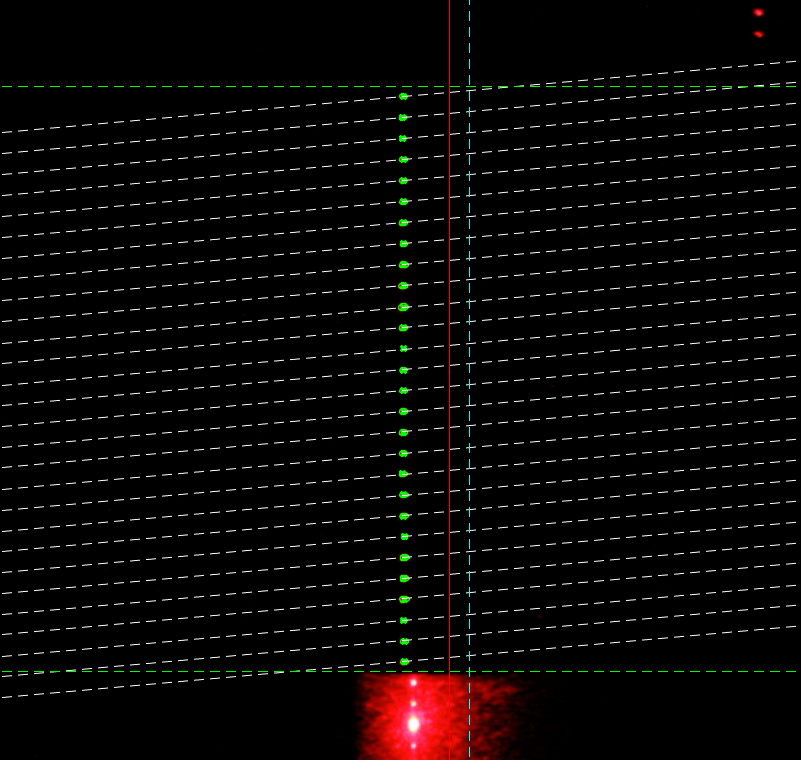
\includegraphics[width=1.0\textwidth]{figures/reconstruction/crossepilines1_crop.png}
        \caption{Frame from the video capture }
    \label{fig:crossepilines1}
    \end{minipage}%
    \hspace{.03\textwidth}
    \begin{minipage}[t]{0.48\textwidth}
        \centering
        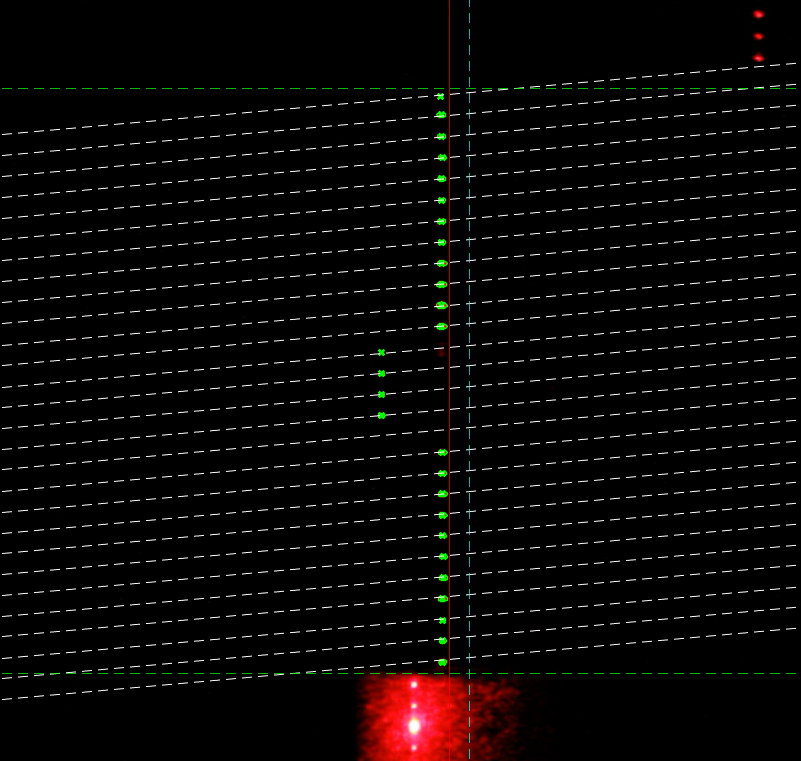
\includegraphics[width=1.0\textwidth]{figures/reconstruction/crossepilines2_crop.png}
        \caption{Frame from the video capture }
        \label{fig:crossepilines2}
    \end{minipage}
\end{figure}
The point cloud reconstruction of the cross shaped object can be seen in figure \ref{fig:crossPC1}.
\begin{figure}[H]
    \centering
    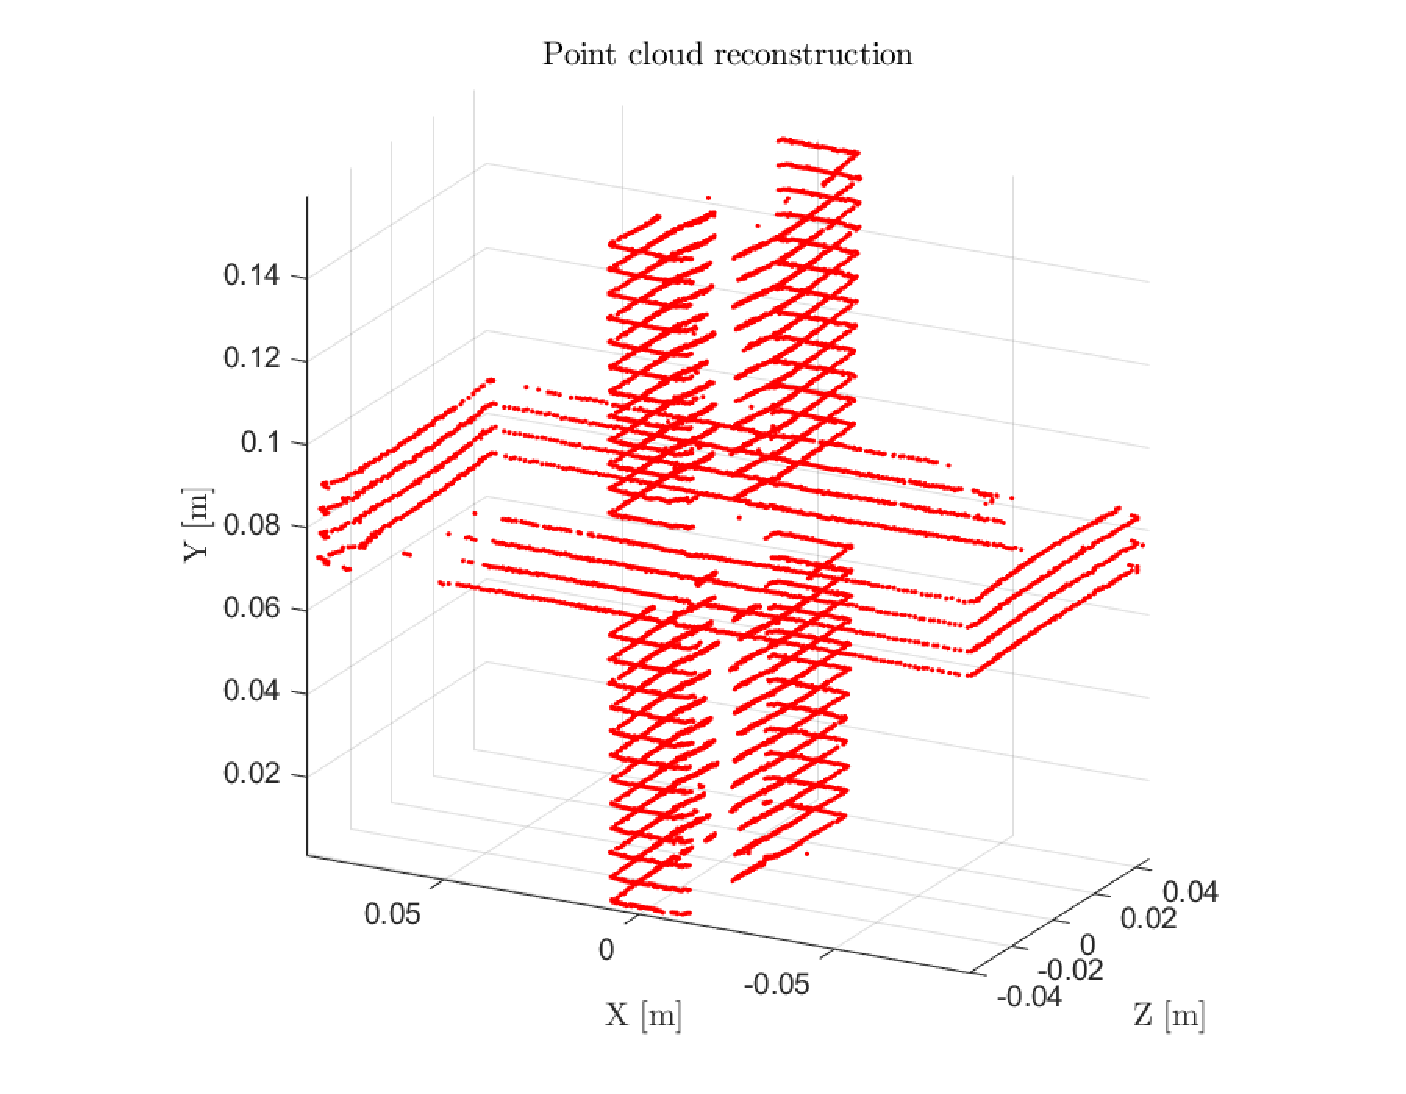
\includegraphics[width=0.95\textwidth]{figures/reconstruction/crossPC1.pdf}
    \caption{Point cloud reconstruction of the cross-shaped object}
    \label{fig:crossPC1}
\end{figure}

From figure \ref{fig:crossPC1} it can be seen that each laser dot creates a horizontal plane of depth values which together outlines the shape of the object. Despite larger holes in the 3D reconstruction, the shape is easily distinguishable and appear to have approximately the same dimensions as illustrated in \ref{fig:crossdimensions}. In this case, the holes in the reconstruction occur due to both occlusions and due to the reflective properties of the object surface which from certain angles can make the laser dots appear very faint, thus hindering the boundary algorithm from correctly detecting the outline of some laser dots.\\

To give the reader a better sense of scale of the reconstruction, the same point cloud is seen in figures \ref{fig:crossPC2} and \ref{fig:crossPC3} from the principal $z$- and $y$-axis, respectively.

\begin{figure}[H]
    \centering
    \begin{minipage}[t]{0.48\textwidth}
        \centering
        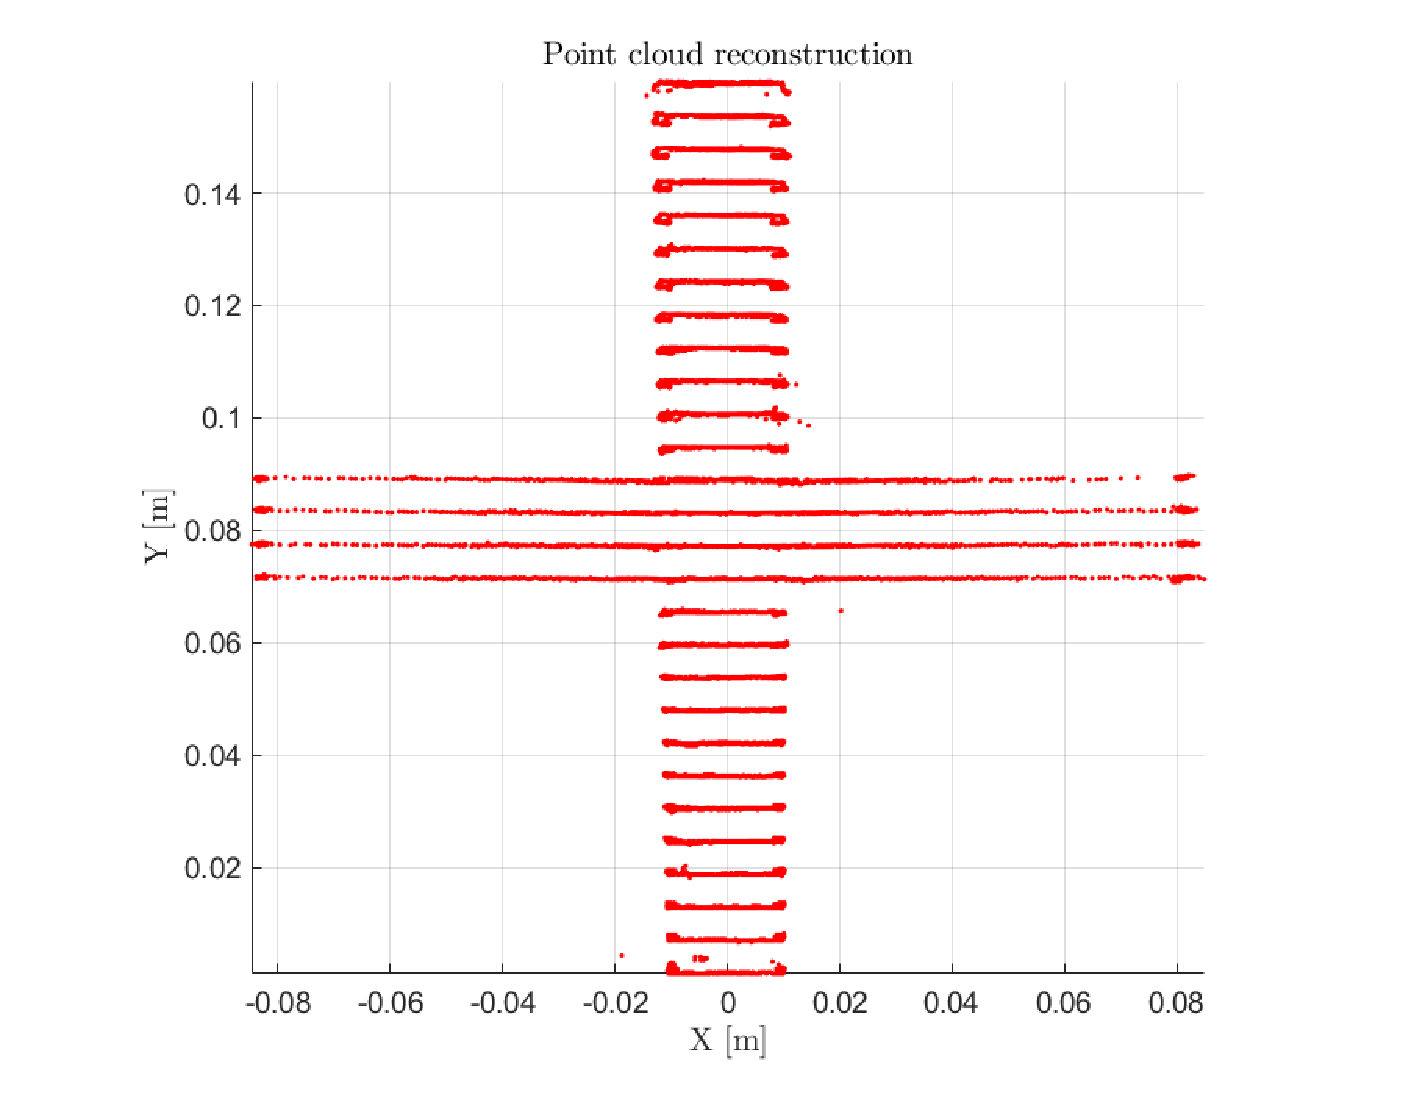
\includegraphics[width=1.25\textwidth]{figures/reconstruction/crossPC2.pdf}
        \caption{Seen from the principal $z$-axis }
    \label{fig:crossPC2}
    \end{minipage}%
    \hspace{.03\textwidth}
    \begin{minipage}[t]{0.48\textwidth}
        \centering
        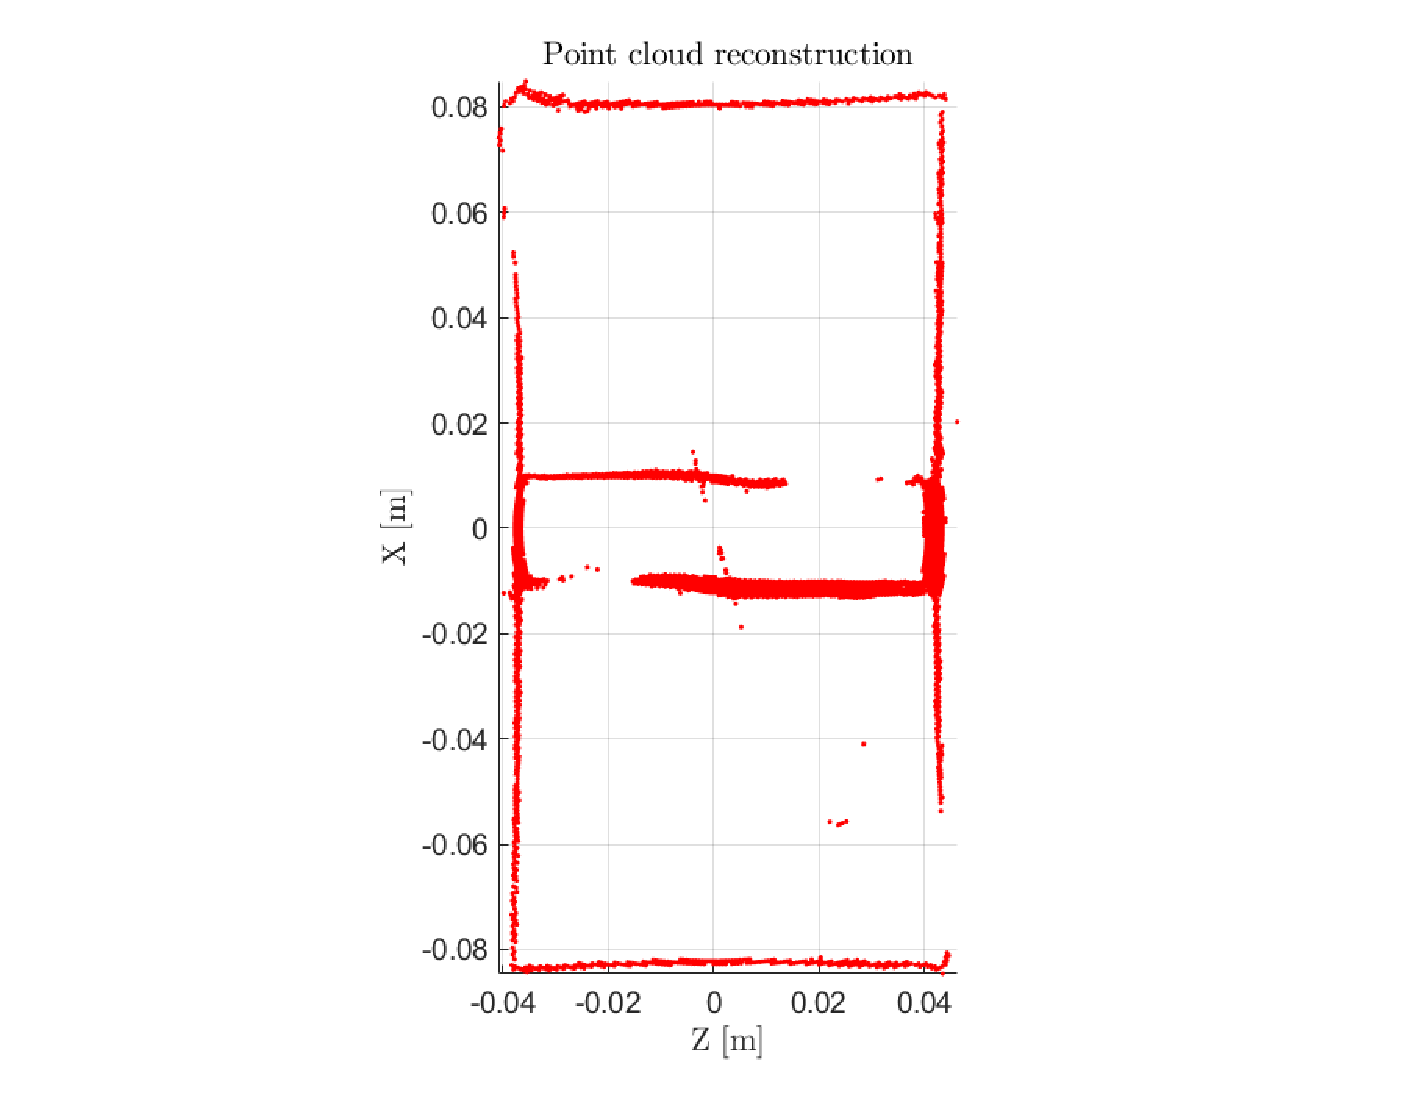
\includegraphics[width=1.25\textwidth]{figures/reconstruction/crossPC3.pdf}
        \caption{Seen from the principal $y$-axis}
        \label{fig:crossPC3}
    \end{minipage}
\end{figure}

Looking at figures \ref{fig:crossPC2} and \ref{fig:crossPC3} and comparing with the illustration in figure \ref{fig:crossdimensions} it can be seen that the reconstructed dimensions are in fact very similar to the ground truth apart from some noise around the edges. The reconstructed object is about 16.5cm in width, about 16cm in height and approximately 8cm in depth as seen from above. These dimensions correspond quite well with the real world dimensions.\\

Next, another slightly more complex object is reconstructed using the exact same method. This time, object of interest is a collection of wooden blocks stacked together. The object consists of a triangular shaped block, three rectangular blocks and a cylinder in the middle. The dimensions of this object are illustrated in figure \ref{fig:wooddimensions}. Note that as before the illustration is not completely to scale. 

\begin{figure}[H]
    \centering
    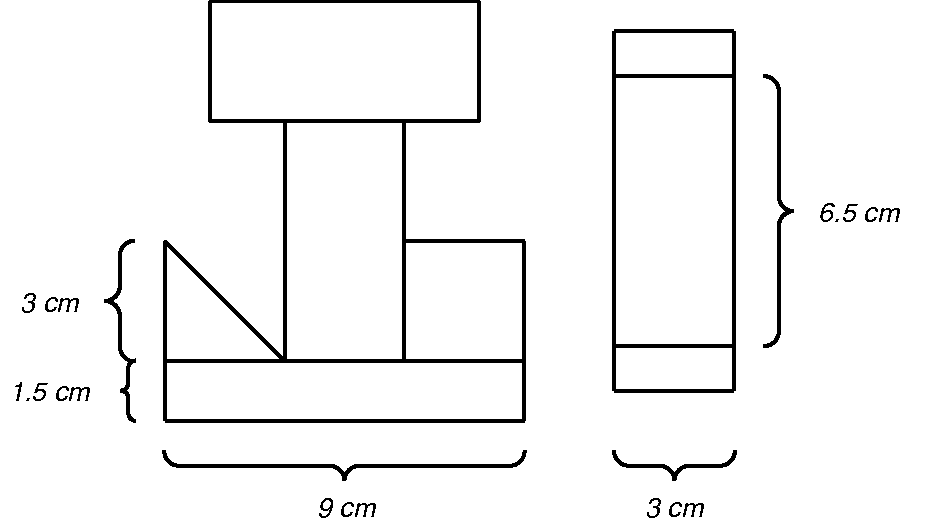
\includegraphics[width=0.7\textwidth]{figures/reconstruction/wooddimensions.pdf}
    \caption{Illustration of the stack of wooden blocks showing the dimensions. The left subplot shows the object from the front and the right shows the object from above.}
    \label{fig:wooddimensions}
\end{figure}

Similarly for the cross, figures \ref{fig:woodepilines1} and \ref{fig:woodepilines2} shows two different frames from the video footage collected using this object, where the same convention has been used to mark the laser dots, detection boundary, epipolar lines, etc.\\

\begin{figure}[H]
    \centering
    \begin{minipage}[t]{0.48\textwidth}
        \centering
        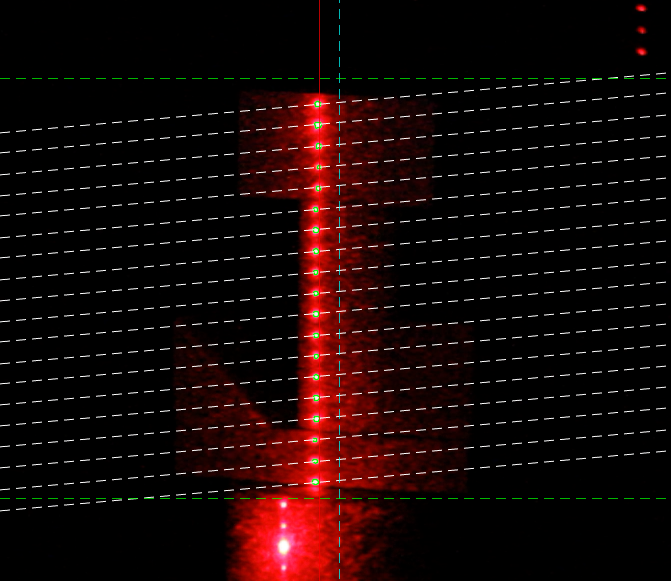
\includegraphics[width=1.0\textwidth]{figures/reconstruction/woodepilines1_crop.png}
        \caption{Frame from the video capture}
    \label{fig:woodepilines1}
    \end{minipage}%
    \hspace{.03\textwidth}
    \begin{minipage}[t]{0.48\textwidth}
        \centering
        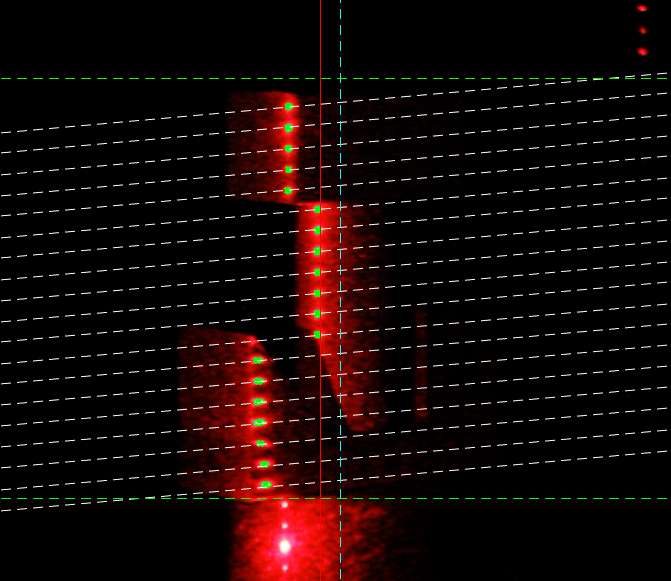
\includegraphics[width=1.0\textwidth]{figures/reconstruction/woodepilines2_crop.png}
        \caption{Frame from the video capture}
        \label{fig:woodepilines2}
    \end{minipage}
\end{figure}

Looking at figures \ref{fig:woodepilines1} and \ref{fig:woodepilines2} it can be seen that the reflective properties of the surface has a large impact on the brightness of the laser dots projected onto the object. In this case, the light from each dot bleeds much more into one another which causes most of object to be lit up in red. As such, a HSV thresholding operation as well as morphological closing was needed to be applied before the boundary algorithm was used on the image, which then yielded reliable centroid estimation of the laser dots. Similarly for the cross, the laser dots move perfectly along the epipolar lines.\\

The point cloud reconstruction of the object illustrated in figure \ref{fig:wooddimensions} can be seen in figure \ref{fig:woodPC1}. In figures \ref{fig:woodPC2} and \ref{fig:woodPC3} the same point cloud can be seen from the principal $z$- and $y$-axis, respectively.

\begin{figure}[H]
    \centering
    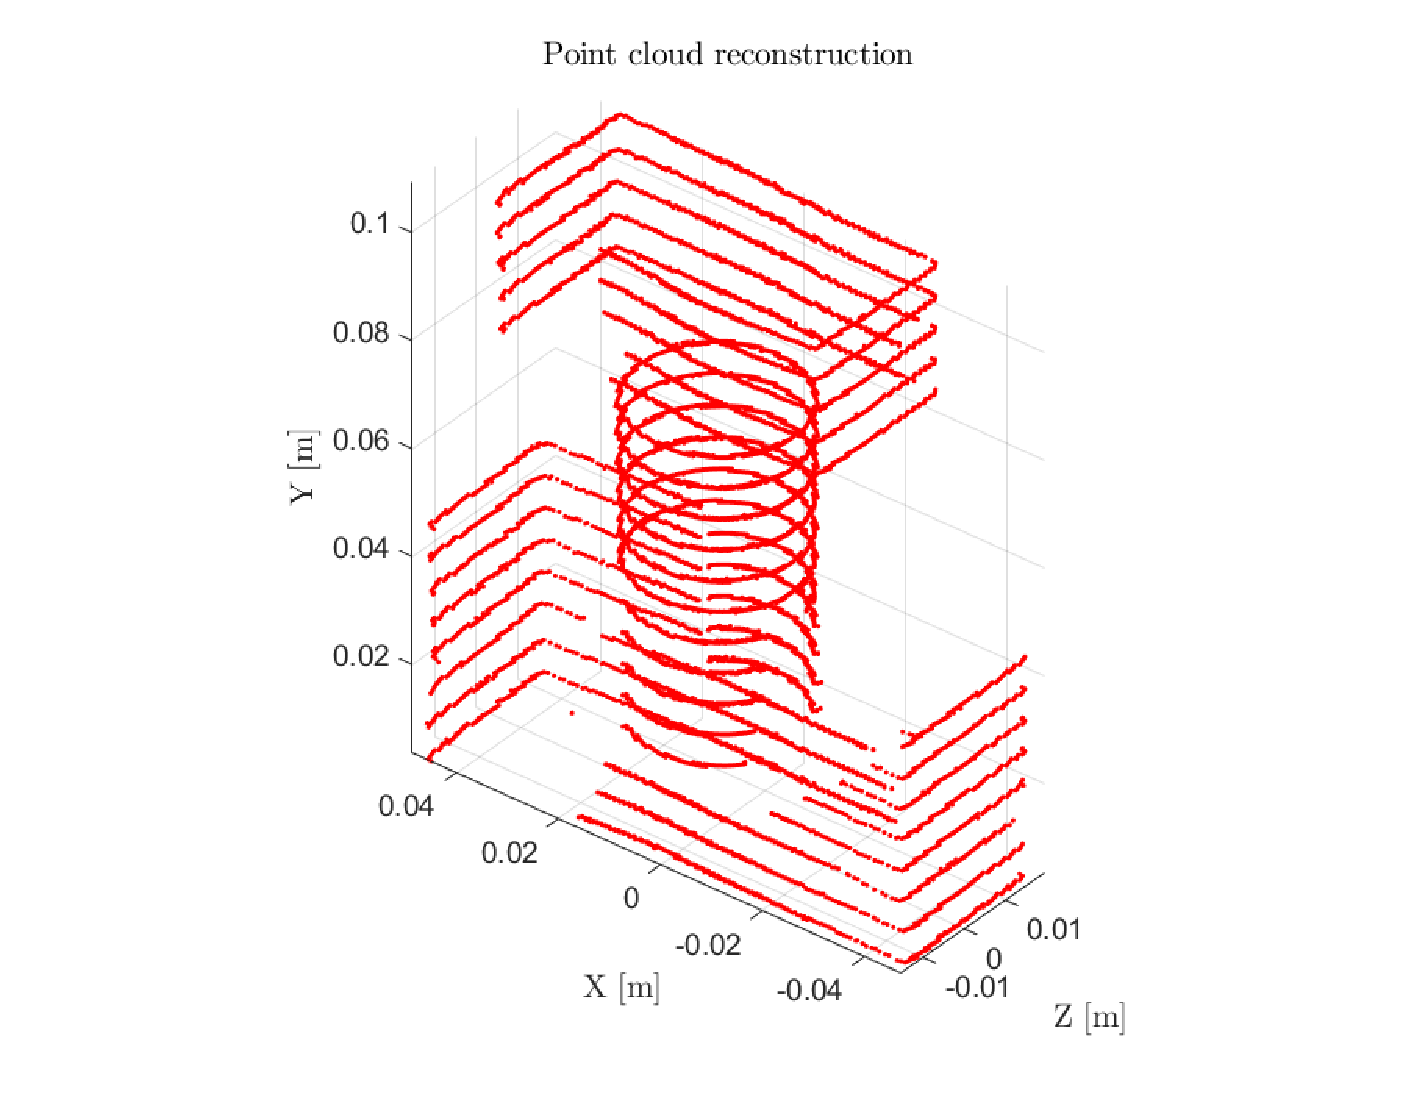
\includegraphics[width=0.95\textwidth]{figures/reconstruction/woodPC1.pdf}
    \caption{Point cloud reconstruction of the stack of wooden blocks}
    \label{fig:woodPC1}
\end{figure}

\begin{figure}[H]
    \centering
    \begin{minipage}[t]{0.48\textwidth}
        \centering
        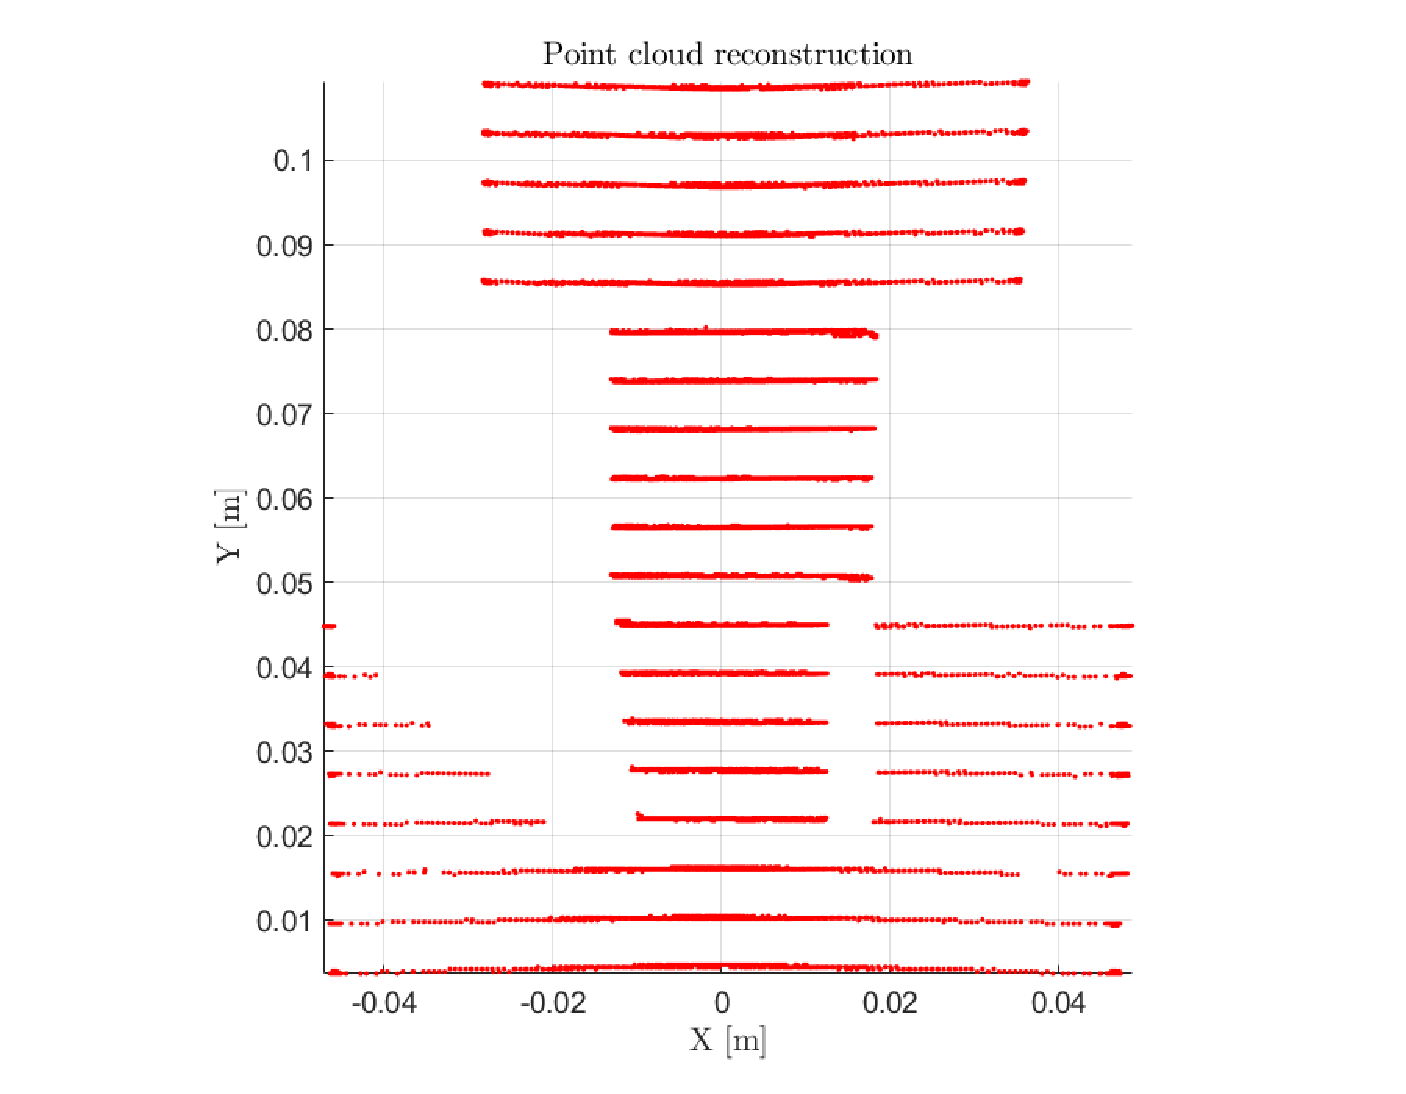
\includegraphics[width=1.25\textwidth]{figures/reconstruction/woodPC2.pdf}
        \caption{Seen from the principal $z$-axis}
    \label{fig:woodPC3}
    \end{minipage}%
    \hspace{.03\textwidth}
    \begin{minipage}[t]{0.48\textwidth}
        \centering
        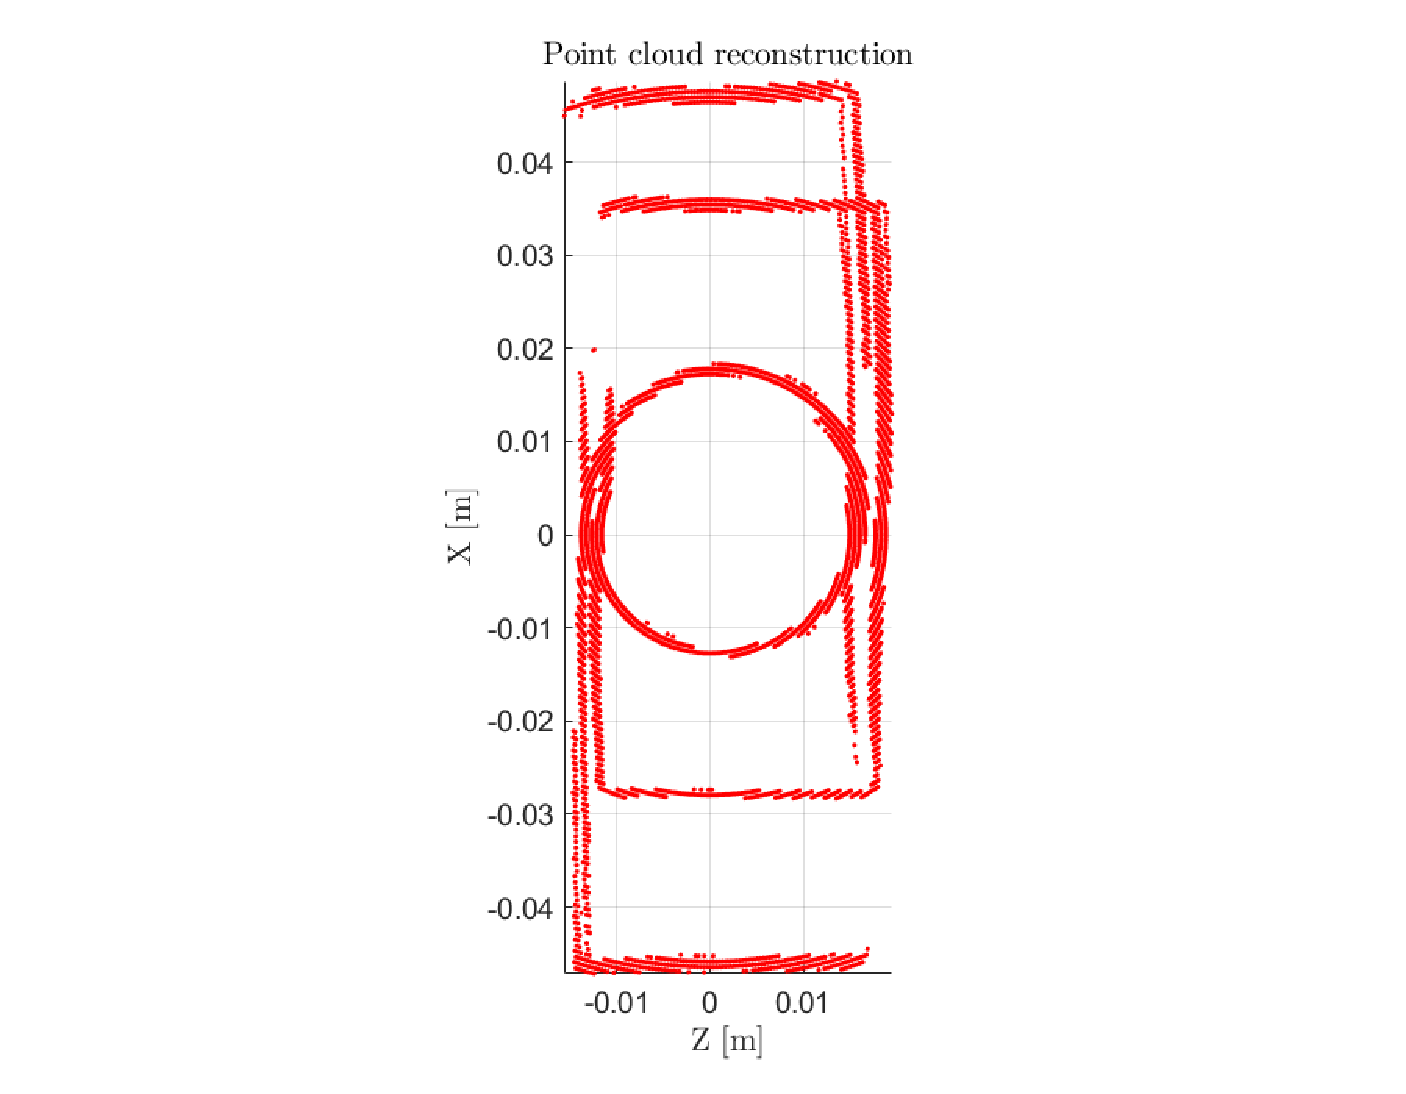
\includegraphics[width=1.25\textwidth]{figures/reconstruction/woodPC3.pdf}
        \caption{Seen from the principal $y$-axis}
        \label{fig:woodPC2}
    \end{minipage}
\end{figure}

Looking at the point cloud in figures \ref{fig:woodPC1}, \ref{fig:woodPC2} and \ref{fig:woodPC3} and comparing with the illustration in figure \ref{fig:wooddimensions} it can be seen that the 3D reconstruction is quite close to the ground truth apart for gaps. The gaps occur due to the shape of the object which the dots at certain angles. Despite this, however, the object is still distinguishable.  
